\documentclass[a4paper]{article}
\usepackage{header}

\setlength{\parindent}{1.5em}
\setlength{\parskip}{0.45\baselineskip plus 0.1\baselineskip minus 0.05\baselineskip}
\let\defaulttableofcontents\tableofcontents
\renewcommand{\tableofcontents}{%
  \begingroup
  \setlength{\parskip}{0pt}%
  \defaulttableofcontents
  \endgroup
}

\begin{document}
\title{\LARGE{Алгоритмы и структуры данных—1}\\ Коллоквиум\\ Материалы для подготовки}
\author{Винер Даниил \href{https://t.me/danya_vin}{@danya\_vin}}
\date{Версия от \today}
\maketitle
Материал в этом файле задает базовый минимум знаний, необходимых для коллоквиума. Принимающий может проверять не только знание изложенных тем, но и глубину их понимания с помощью уточняющих вопросов.
\tableofcontents
\newpage
\section{Способы задания графов}
Любой граф $G$ можно представить двумя множествами: $V$ — множество вершин, $E$ — множество рёбер. Будем обозначать $n=|V|$ — количество вершин, $m=|E|$ — количество рёбер.

\subsection{Список ребер}
\definition Список ребер — структура данных, представляющая собой набор из пар $A_i-B_i$, где $A_i,B_i$ — вершины графа

Порядок в списке ребер не важен \textbf{только в случае неориентированных} графов

\subsubsection*{Сложность нахождения всех соседей каждой вершины}
Если граф неориентирован, то оптимально будет сделать его ориентированным (помимо ребра $A_i-B_i$ добавить ребро $B_i-A_i$)

\begin{itemize}
    \item Для поиска всех соседей вершины (в неориентированном случае) надо перебрать все ребра и сравнить текущую вершину со второй вершиной ребра. $O(m)$
    \item Сортировка ребер — $O(m\log m)$
    \item Поиск первого соседа в списке ребер для одной вершины — $O(\log m)$
    \item Поиск первого соседа в списке ребер для всех — $O(n\log m)$
\end{itemize}

Так как обычно в графах $m\geqslant n$, то для поиска всех соседей всех вершин потребуется $O(m\log m)$

\subsection{Матрица смежности}
\textbf{Матрица смежности} — матрица графа $G=(V,E)$ размера $n\times n$, такая что на пересечении $i$-й строки и $j$-го столбца стоит 1, если есть ребро между вершинами $i$ и $j$, и 0 иначе

Если граф ориентированный, то $A[i][j]=1$ означает наличие ребра $i\to j$. Для неориентированного графа матрица смежности симметрична относительно главной диагонали.

Имея граф, заданный матрицей смежности, можно выполнить такие операции:
\begin{itemize}
    \item Проверить наличие ребра между двумя вершинами за $O(1)$
    \item Найти всех соседей одной вершины за $O(n)$
    \item Просмотреть все рёбра графа за $O(n^2)$
\end{itemize}

\textbf{Затраты по памяти} — $O(n^2)$, так как храним матрицу размера $n\times n$

\subsection{Список смежности}
\textbf{Список смежности} — массив, в котором каждой вершине графа соответствует список, состоящий из соседей этой вершины

Изначально создается $n$ динамически расширяемых пустых векторов. При считывании ребра $A_i-B_i$ в вектор с номером $A_i$ добавляется ребро $B_i$ (если граф неориентированный, то еще в вектор с номером $B_i$ добавляется ребро $A_i$)

\textbf{Сложность построения} — $O(n+m)$, так как нужно создать $n$ списков и добавить $m$ рёбер. Если пустые списки уже созданы, добавление всех рёбер занимает $O(m)$

\textbf{Сложность нахождения всех соседей вершины} — $O(\deg v)$, где $\deg v$ — степень вершины $v$

\textbf{Сложность нахождения всех соседей каждой вершины} — $O(n+m)$, так как мы проходим по всем вершинам за $n$ и просматриваем каждое ребро за $m$

\textbf{Затраты по памяти} — $O(n+m)$

\newpage
\section{Обход в глубину}
\subsection{Обход в глубину}
\subsubsection*{Описание алгоритма}
Обход начинается с выбранной стартовой вершины. Из текущей вершины алгоритм переходит в одного из непосещенных соседей. Если у вершины не осталось непосещенных соседей, то алгоритм возвращается назад по текущему пути, пока не найдет вершину, из которой можно продолжить обход.

\textbf{Рекурсивная реализация.} При входе в вершину $v$ помечаем ее посещенной. Затем перебираем всех соседей $to$ вершины $v$; если сосед еще не посещен, рекурсивно запускаем DFS из $to$. Когда у вершины не остается непосещенных соседей, рекурсивный вызов завершается, и управление возвращается к предыдущей вершине в текущем пути.

\textbf{Итеративная реализация на стеке.} В стек кладем стартовую вершину и помечаем ее посещенной. Пока стек не пуст, смотрим на вершину $v$ наверху стека. Если у $v$ есть непосещенный сосед $to$, помечаем $to$ посещенным и кладем его в стек. Если таких соседей нет, удаляем $v$ из стека и возвращаемся к предыдущей вершине. Так стек явно хранит текущий путь обхода и заменяет стек рекурсивных вызовов. Чтобы не перебирать одних и тех же соседей заново, для каждой вершины хранят номер следующего рассматриваемого соседа или кладут в стек пару из вершины и этого номера.

Отметим, что в общем случае, когда неизвестно, связный граф или нет, нужно запустить обход в цикле по всем вершинам: новый запуск начинается из каждой еще непосещенной вершины

\subsubsection*{Применение алгоритма}
\begin{enumerate}
    \item Поиск случайного пути в лабиринте
    \item Решение задач, связанных с построением маршрута: в сети, на карте, в сервисах покупки билетов и так далее
    \item Проверка на наличие циклов, топологическая сортировка
\end{enumerate}

\subsubsection*{Асимптотика}
\label{dfs_asimp}
\textbf{Дополнительная память DFS} — $O(V)$, где $V$ — количество вершин графа. Эта оценка учитывает массив посещенности и стек рекурсии или явный стек, но не учитывает память на хранение самого графа.

Временная сложность зависит от представления графа: матрица смежности, список ребер или список смежности. Рассмотрим каждый вариант:

\begin{enumerate}
    \item Список смежности — $O(V+E)$
    \begin{itemize}
        \item Вершины посещаются (проверяются на посещенность) только один раз, что составляет $O(V)$
        \item Суммарно просматриваются все записи списков смежности: в ориентированном графе это $E$ записей, а в неориентированном — $2E$, что все равно составляет $O(E)$
    \end{itemize}
    \item Матрица смежности — $O(V^2)$
    \begin{itemize}
        \item Для каждой посещенной вершины приходится просматривать строку матрицы длины $V$; при обходе всех компонент таких строк не больше $V$
    \end{itemize}
    \item Список рёбер
    \begin{itemize}
        \item Без предварительной обработки для поиска соседей текущей вершины приходится просматривать весь список рёбер, поэтому полный обход может занять $O(VE)$
        \item Обычно перед DFS по списку рёбер строят список смежности за $O(V+E)$, после чего сам обход работает за $O(V+E)$
        \item Если хранить отсортированный список рёбер и искать диапазон исходящих рёбер бинарным поиском, то с учетом сортировки получается $O(E\log E + V\log E + E)$
    \end{itemize}
\end{enumerate}

\subsubsection*{Пример}
\begin{center}
    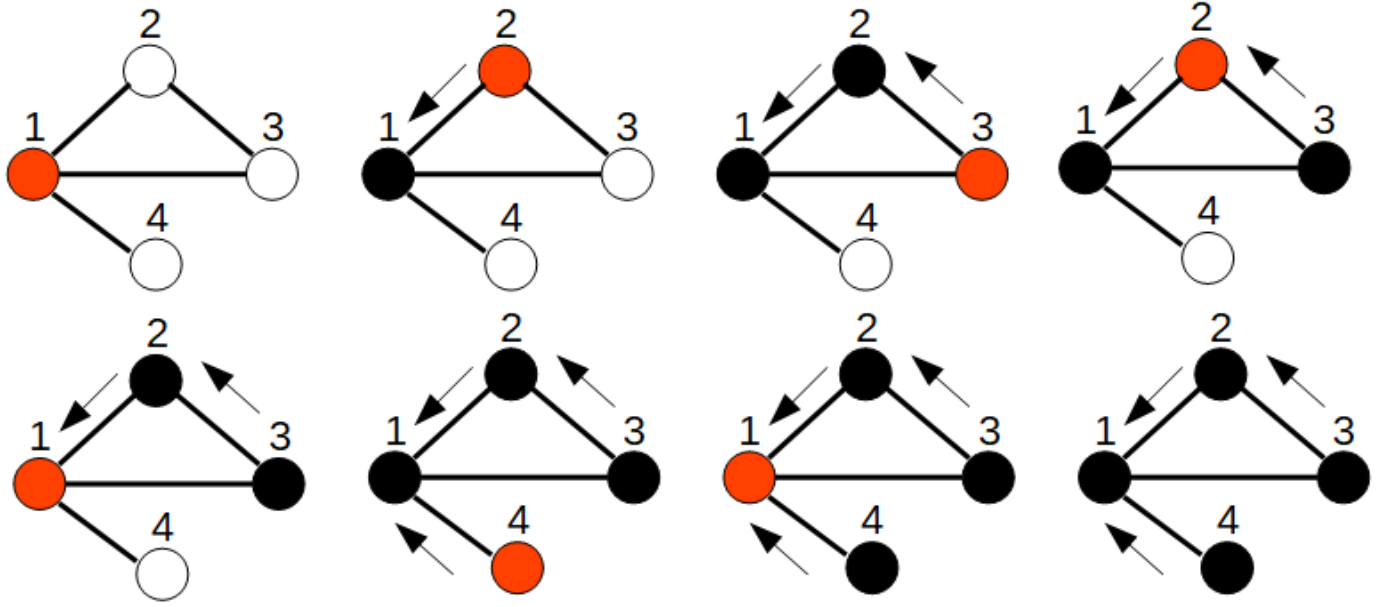
\includegraphics[width=0.8\linewidth]{img/dfs.png}
    \label{dfs}
\end{center}
% \subsubsection*{Псевдокод}
% \begin{lstlisting}
% void dfs(int v){
%     used[v] = 1;
%     for (auto to : gr[v]){
%         if (!used[to]){
%             dfs(to);
%         }
%     }
% }
% \end{lstlisting}

\subsection{Связность неориентированного графа}
\textbf{Связный граф} — граф, в котором существует путь от любой вершины до любой другой вершины

\subsubsection*{Проверка неориентированного графа на связность}
Запуск DFS от любой из вершин графа

\begin{itemize}
    \item Запускаем DFS из любой вершины
    \item После DFS проверяем, посещены ли все вершины. Если да — граф связный, нет — несвязный
    \item Дополнительная память — $O(V)$ под массив посещенности и стек рекурсии или явный стек, плюс хранение графа
    \item Сложность по времени при хранении графа списком смежности — $O(V+E)$
\end{itemize}

\subsection{Сильная связность ориентированного графа}
\definition В ориентированном графе сильная связность требует, чтобы для любых двух вершин $u$ и $v$ существовал ориентированный путь $u\rightarrow v$ и $v\rightarrow u$

Для проверки нужно выполнить два запуска DFS

\begin{enumerate}
    \item Запускаем DFS на исходном графе
    \begin{itemize}
        \item Выбираем любую вершину $v$
        \item Запускаем из неё DFS, помечая все достижимые вершины
        \item После завершения проверяем: если посетили не все $V$ вершин, то граф не сильно связен
    \end{itemize}
    \item Второй запуск DFS в транспонированном графе
    \begin{itemize}
        \item Строим транспонированный граф, то есть все ребра $u\rightarrow v$ превращаются в $v\rightarrow u$
        \item Запускаем DFS из той же вершины $v$
        \item Снова убеждаемся, что посетили все вершины
    \end{itemize}
\end{enumerate}

Если во время обоих обходов мы посетили все вершины, то граф является сильно связным

\textbf{Временная сложность:} $O(V+E)$ при хранении графа списком смежности, так как построение транспонированного графа и каждый из двух запусков DFS занимают линейное время.

\textbf{Дополнительная память:} $O(V+E)$, если транспонированный граф строится явно. Без учета транспонированного графа сами обходы требуют $O(V)$ памяти.

\subsection{Поиск компонент связности в графе}
\textbf{Компонента связности неориентированного графа} — максимальное по включению подмножество вершин и соединяющих их ребер, такое что есть путь из каждой вершины в каждую

\subsubsection*{Алгоритм поиска компоненты связности}
Можно раскрасить граф в компоненты связности. Каждой вершине ставится в соответствие номер компоненты связности, к которой относится вершина

\textbf{Реализация происходит через DFS}

Может потребоваться несколько запусков поиска в глубину. Поэтому поиск проводим через цикл, перебирающий все вершины

\begin{itemize}
    \item Заводим массив длины $V$ для хранения цвета каждой вершины
    \item При входе в DFS красим вершину в текущий цвет (\code{color[v] = component})
    \item Если очередная вершина не покрашена, то счетчик количества компонент связности увеличивается и запускается DFS для этой вершины со значением цвета равным текущему значению счетчика
\end{itemize}

\textbf{Затраты по памяти} составят $O(V)$ под массив цветов и стек рекурсии (или стек при итеративном обходе), плюс хранение графа

\textbf{Сложность по времени:} $O(V + E)$ при хранении графа списком смежности, потому что каждая вершина красится один раз, а суммарно по всем запускам DFS просматриваются все записи списков смежности. Цикл по всем вершинам добавляет только $O(V)$ проверок цвета.

\subsection{Поиск цикла в графе}
Описанный ниже способ с серыми вершинами используется для поиска цикла в ориентированном графе. Чтобы найти цикл, нужно раскрасить граф в три цвета:

\begin{itemize}
    \item \textbf{Белый} — вершина не посещена
    \item \textbf{Серый} — DFS вошел в вершину, но не обработал всех соседей
    \item \textbf{Черный} — все соседи вершины посещены и помечены черным
\end{itemize}

\[
    \boxed{\text{Обратное ребро в серую вершину означает, что в ориентированном графе есть цикл}}
\]

Для неориентированного графа нужно учитывать, что ребро из вершины в ее родителя в дереве DFS не образует цикл. Поэтому при просмотре соседа $to$ вершины $v$ цикл найден только если $to$ уже посещен и $to \neq parent[v]$.

Если нужно проверить весь граф, а не только одну достижимую часть, DFS запускают в цикле из всех еще не посещенных вершин.


\subsubsection*{Алгоритм}
\begin{itemize}
    \item В каждый момент времени серым цветом будут помечены вершины, лежащие на пути \dfs от стартовой вершины до текущей
    \item Если из текущей вершины $u$ есть ребро в серую вершину $v$, то в графе есть цикл, так как существует путь от $v$ до $u$ ($v$ лежит на пути от стартовой вершины до $u$) и путь от $u$ до $v$, проходящий по одному ребру
\end{itemize}

\textbf{Временная сложность:} $O(V + E)$ при хранении графа списком смежности, поскольку каждая вершина и каждая запись в списках смежности обрабатываются не более одного раза

\textbf{Память:} $O(V)$ под массив меток и стек рекурсии или явный стек, плюс хранение графа.

\subsubsection*{Восстановление цикла}
Допустим, для $u$ нашелся серый сосед $v$, тогда запоминаем номер $v$ и выходим из рекурсивной функции, запоминая номера вершин, пока не дойдем до вершины, в которой нашелся цикл 
 
\subsection{Проверка графа на двудольность}
\textit{Примечание.} Граф — двудольный тогда и только тогда, когда все циклы в графе имеют четную длину

\textbf{Алгоритм}

\begin{itemize}
    \item Выбираем произвольную вершину и красим ее в цвет \textit{color}
    \item Всех соседей этой вершины красим в цвет $3-color$
    \item Соседей соседей — в цвет \textit{color} и т.д.
    \item Если в какой-то момент сосед вершины уже покрашен в тот же цвет, что и вершина, то алгоритм завершает работу, так как граф не двудольный, потому что есть циклы нечетной длины
\end{itemize}

Если граф не является связным, то нужно запустить \dfs из каждой вершины каждой компоненты связности (как в разделе про поиск компонент связности)

\textbf{Временная сложность:} $O(V+E)$ при хранении графа списком смежности, потому что каждая вершина получает цвет один раз, а каждое ребро проверяется при просмотре списков смежности.

\textbf{Память:} $O(V)$ под массив цветов и стек рекурсии или явный стек, плюс хранение графа.


\subsection{Диаметр и центр дерева}
\textbf{Диаметр дерева} — максимальная длина (в рёбрах) кратчайшего пути в дереве между любыми двумя вершинами

\textbf{Центр дерева} — одна вершина или две соседние вершины, минимизирующие максимальное расстояние до всех остальных вершин

\textit{Примечание.} Центр можно понимать так: это вершина дерева, такая что при подвешивании дерева за нее глубина дерева минимальна

\subsubsection*{Алгоритм поиска диаметра дерева}
Для поиска диаметра требуется выполнить два запуска DFS. Этот алгоритм работает именно для дерева.

\begin{itemize}
    \item Берем любую вершину дерева (пусть это $a$) и ищем самую удаленную от нее вершину $b$ с помощью \dfs
    \item Из вершины $b$ запускаем \dfs и ищем самую удаленную от нее вершину (пусть это $c$)
    \item Путь из $b$ в $c$ — диаметр дерева
\end{itemize}

Центр дерева находится как середина найденного диаметрального пути: если длина пути в ребрах четная, центр один; если нечетная, центров две соседние вершины.

\textbf{Временная сложность:} $O(V+E)=O(V)$, потому что в дереве $E=V-1$, а алгоритм выполняет два DFS и затем один раз просматривает найденный путь.

\textbf{Память:} $O(V)$ под массив посещенности, массив предков для восстановления пути и стек рекурсии или явный стек, плюс хранение дерева.

% \begin{lstlisting}
%     std::vector<node> find_diameter() {
%         std::vector<node> ans, path;
%         std::vector<int> used(gr_.size(), 0);

%         std::function<void(node v)> dfs = [&] (node v) {
%             used[v] = true;
%             path.emplace_back(v);
%             for (const auto& to : gr_[v]) {
%                 if (!used[to]) {
%                     dfs(to);
%                 }
%             }
%             if (ans.size() < path.size()) {
%                 ans = path;
%             }
%             path.pop_back();
%         };
%         dfs(0);
%         used.assign(gr_.size(), 0);
%         dfs(ans.back());
%         return ans;
%     }
% \end{lstlisting}

\newpage
\section{Задача построения дерева кратчайших расстояний}
\subsection{Обход в ширину}
\subsubsection*{Наивный алгоритм}
Создаем массив расстояний, заполняем его бесконечностями. Для начальной вершины установим значение 0

Делаем шаги по расстояниям, пока есть вершины текущего слоя. На каждом шаге перебираем все вершины, выбираем те, расстояние до которых равно номеру текущего слоя, и помечаем их еще не посещенных соседей числом на 1 большим, чем номер текущего слоя

\begin{itemize}
    \item На нулевом шаге выбираем начальную вершину и помечаем ее соседей 1
    \item Затем выбираем вершины, находящиеся на расстоянии 1, и их непомеченных соседей помечаем 2 и т.д.
\end{itemize}

\textbf{Сложность по времени} — $O(V^2+E)$, так как мы сделаем не более $V$ шагов, на каждом шаге переберем $V$ вершин, а также суммарно просмотрим все рёбра

\textbf{Сложность по памяти} — $O(V)$ заводится под массив расстояний

\subsubsection*{Реализация через очередь}
\begin{enumerate}
    \item Инициализировать для всех $u$: $\text{dist}[u]=\infty$, $\text{visited}[u]=\text{false}$
    \item $\text{dist}[start]=0$, $\text{visited}[start]=\text{true}$, положить $start$ в очередь $q$
    \item Пока $q$ не пуста:
    \begin{itemize}
        \item $u = q.\text{pop}()$
        \item Для каждого соседа $v$ из $\mathrm{adj}[u]$:
        \begin{itemize}
            \item Если $\neg\text{visited}[v]$:
            \begin{itemize}
                \item $\text{visited}[v]=\text{true}$
                \item $\text{dist}[v]=\text{dist}[u]+1$
                \item $q.\text{push}(v)$
                \item Если $v$ — искомая вершина, выйти из всех циклов (если ищем путь до конкретной вершины)
            \end{itemize}
        \end{itemize}
    \end{itemize}
\end{enumerate}

\textbf{Сложности:}
\begin{itemize}
    \item Время: $O(V + E)$
    \item Память: $O(V)$ под очередь, массивы \texttt{dist} и \texttt{visited}, плюс хранение графа
\end{itemize}

% \subsubsection*{Применение алгоритма}
% \begin{enumerate}
%     \item Для поиска кратчайшего пути в неявно заданных и невзвешенных графах
%     \item Для обнаружения кратчайших путей и минимальных покрывающих деревьев
%     % \item Для построения индексов веб-страниц
% \end{enumerate}

\textit{Белый} — еще не посещенные вершины, \textit{черный} — уже посещенный, \textit{красный} — обрабатывающиеся в данный момент (в начале очереди), \textit{серый} — вершины, находящиеся в очереди

\begin{center}
    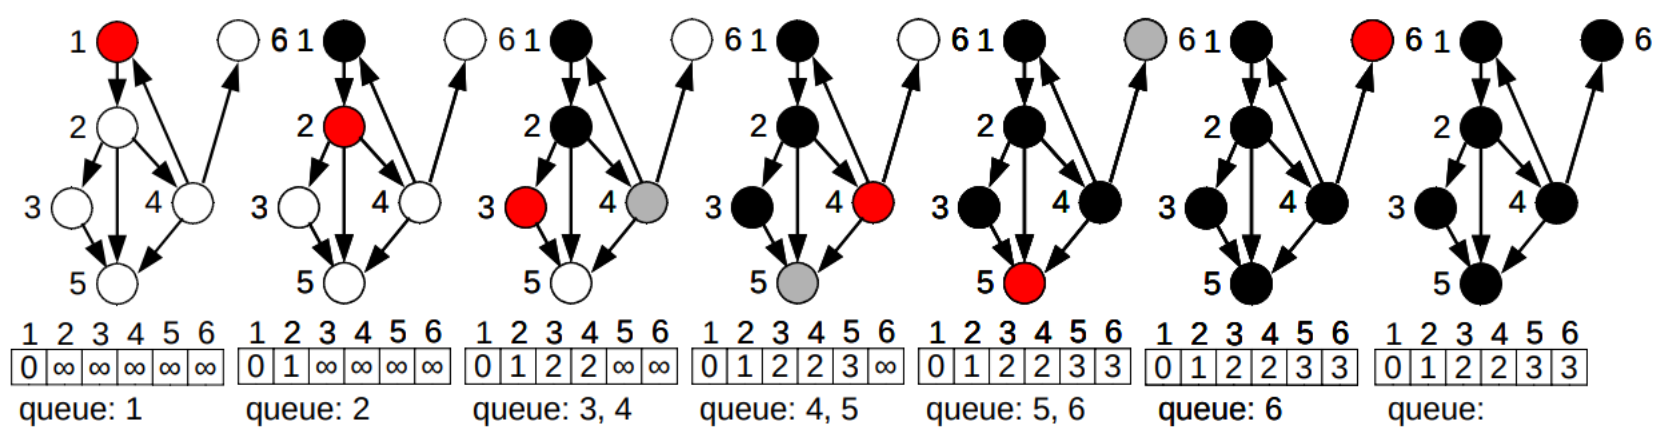
\includegraphics[width=1\linewidth]{img/bfs.png}
    \label{bfs}
\end{center}

\subsection{Алгоритм Дейкстры}
\textit{Важно.} Веса рёбер должны быть неотрицательными, иначе алгоритм не будет работать корректно

\subsubsection*{Случай для плотного графа}
Создадим такие массивы

\begin{itemize}
    \item \code{dist} — размером $V+1$. В нем для каждой вершины хранится текущая длина кратчайшего пути от начальной вершины $s$. (\code{dist[s] = 0}, а все остальное — $\infty$)
    \item \code{visited} — размером $V+1$. Хранит информацию о том, обработана вершина или нет
\end{itemize}

Алгоритм состоит не более чем из $V$ шагов. На каждом шаге делаем следующее

Для $i=1\ldots V$:
\begin{enumerate}
    \item Выбрать необработанную вершину $v$ с минимальным \code{dist[v]}
    \item Если такой вершины нет или \code{dist[v]} равно $\infty$, то все достижимые вершины уже обработаны
    \item Пометить $v$ как обработанную и выполнить релаксацию всех рёбер $(v \to u)$:
    \[
        \code{dist[u]} = \min(\code{dist[u]}, \code{dist[v]} + w(v,u)).
    \]
\end{enumerate}


% \textit{Красный} — вершины, для которых будет произведена релаксация, \textit{серый} — обработанные вершины\\
\begin{center}
    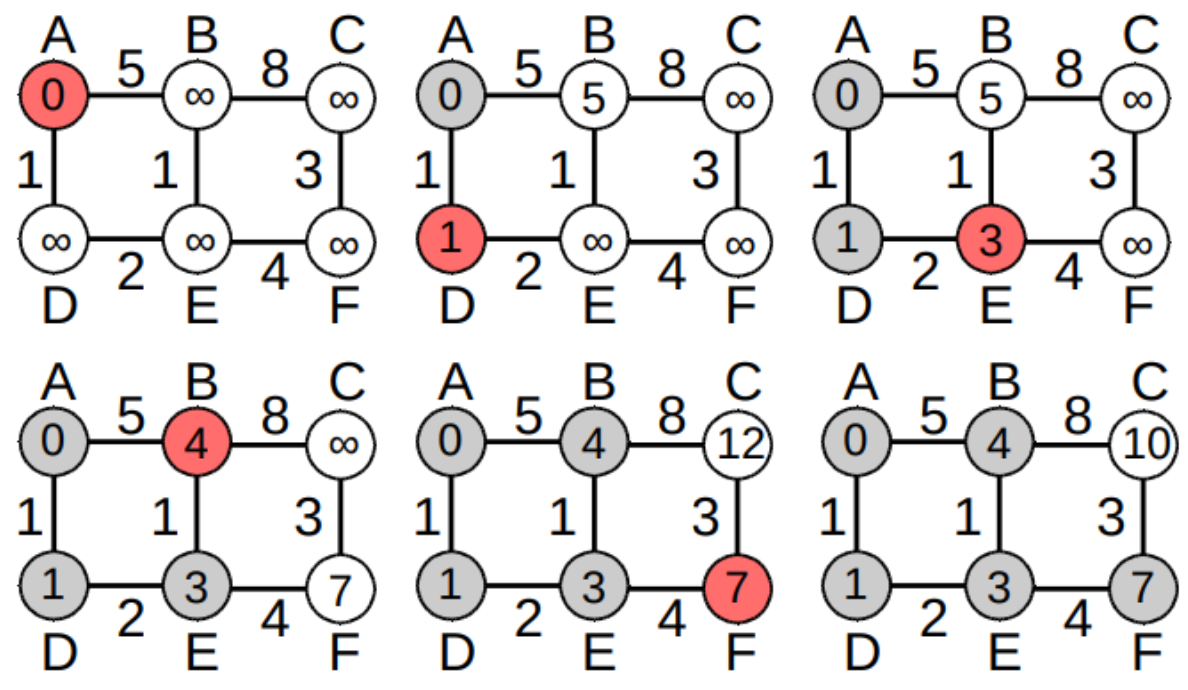
\includegraphics[width=0.8\linewidth]{img/dijkstra.png}
    \label{dijkstra}
\end{center}

\textit{Красный} — вершины, для которых будет произведена релаксация, \textit{серый} — обработанные вершины

\textbf{Сложность со списком смежности} — $O(V^2+E)$, так как мы на каждом из не более чем $V$ шагов ищем минимум из $V$ чисел для вершин и суммарно просматриваем все рёбра

\textbf{Сложность с матрицей смежности} — $O(V^2)$

\subsubsection*{Случай для разреженного графа}
\textit{Напоминание.} Разреженный граф - граф, у которого количество рёбер значительно меньше, чем $V^2$

В разреженном графе минимум среди необработанных вершин удобно искать не линейным проходом, а с помощью структуры данных: \code{ordered set} или очереди с приоритетами.

\begin{enumerate}
    \item Инициализируем расстояния:
    \begin{itemize}
        \item \code{dist[s] = 0}
        \item Для всех остальных вершин \code{dist[v]} равно $\infty$
        \item В структуру данных кладем пару $(0, s)$
    \end{itemize}
    \item Пока структура данных не пуста:
    \begin{itemize}
        \item Достаем вершину $v$ с минимальным текущим расстоянием
        \item Если достали устаревшее значение расстояния, пропускаем его
        \item Для каждого ребра $(v\to u)$ веса $w$ выполняем релаксацию:
        \begin{itemize}
            \item Если \code{dist[u] > dist[v] + w}, то обновляем \code{dist[u]}
            \item В \code{ordered set} удаляем старую пару для $u$ и добавляем новую
            \item В \code{priority queue} просто добавляем новую пару; старые пары будут пропущены, когда окажутся наверху
        \end{itemize}
    \end{itemize}
\end{enumerate}

Процесс повторяется, пока не будут определены кратчайшие пути до всех достижимых вершин.

\textbf{Сложность —} $O((V+E)\log V)$ при использовании \code{ordered set} или кучи с ленивым удалением устаревших значений. Извлечение минимума и обновление структуры данных стоят $O(\log V)$, а каждое ребро может привести не более чем к одной успешной релаксации.

В итоге массив расстояний содержит кратчайшие пути от начальной вершины до всех остальных достижимых вершин.


\subsection{Алгоритм Форда-Беллмана}
Создадим такой массив

\begin{itemize}
    \item \code{dist} — размером $V+1$. Массив кратчайших расстояний. (\code{dist[s] = 0}, а все остальное — $\infty$)
\end{itemize}

Алгоритм состоит из $V-1$ фаз. Пусть есть ребро $(u,v)$ и его вес $w$. На каждой фазе перебираем все рёбра и проводим релаксацию по этому ребру, то есть

\begin{lstlisting}
    if (dist[u] != inf && dist[v] > dist[u] + w){
        dist[v] = dist[u] + w
    }
\end{lstlisting}

\subsubsection*{Проверка отрицательного цикла}
После $V-1$ фаз запускаем еще одну фазу релаксаций. Если на ней расстояние до какой-то вершины снова уменьшилось, то существует отрицательный цикл, достижимый из стартовой вершины. В этом случае кратчайшие расстояния до вершин, на которые влияет этот цикл, не определены.

\subsubsection*{Применение алгоритма}
Алгоритм Форда-Беллмана ищет кратчайшие пути от одной вершины до всех остальных, работает при отрицательных рёбрах и умеет обнаруживать отрицательный цикл, достижимый из стартовой вершины.

\textbf{Временная сложность:} $O(V \times E)$

\textbf{Сложность по памяти:} $O(V + E)$ 

\begin{itemize}
    \item $O(V)$ под массив \texttt{dist}
    \item $O(E)$ под список рёбер
\end{itemize}


\subsection{Алгоритм Флойда–Уоршалла}
Работаем с матрицей размера $V\times V$, где
\[
  \mathrm{dist}[i][j] =
    \begin{cases}
      w(i,j), & \text{если }(i\to j)\text{ есть ребро},\\
      0,      & i=j,\\
      \infty,& \text{иначе}.
    \end{cases}
\]

\textbf{Основной тройной цикл:}

\begin{lstlisting}
    for k in 1..V:
        for i in 1..V:
            for j in 1..V:
                dist[i][j] = min(dist[i][j], dist[i][k] + dist[k][j])

\end{lstlisting}

\textbf{Обнаружение отрицательного цикла:}

Если после выполнения алгоритма \(\mathrm{dist}[i][i]<0\) для некоторого \(i\), в графе есть отрицательный цикл.

\subsubsection*{Применение}
\begin{itemize}
    \item Поиск кратчайших путей «каждый→каждый»
\end{itemize}

\textbf{Сложности:}

\begin{itemize}
    \item Время: \(O(V^3)\)
    \item Память: \(O(V^2)\)
\end{itemize}

\newpage
\section{Задача union — find}
\subsection{Задача union — find}
Пусть у нас есть $N$ элементов, занумерованных от 1 до $N$. Изначально каждый элемент находится в своем отдельном множестве (также занумерованных от 1 до $N$). Нам необходимо поддерживать такие операции:

\begin{itemize}
    \item \code{find(x)} — найти номер множества, в котором лежит $x$
    \item \code{union(x, y)} — объединить множества, содержащие $x$ и $y$
    \item Можно добавить, но необязательно:
    \begin{itemize}
        \item \code{make(x)} — создает новое множество, содержащее $x$ 
    \end{itemize}
\end{itemize}

\begin{center}
    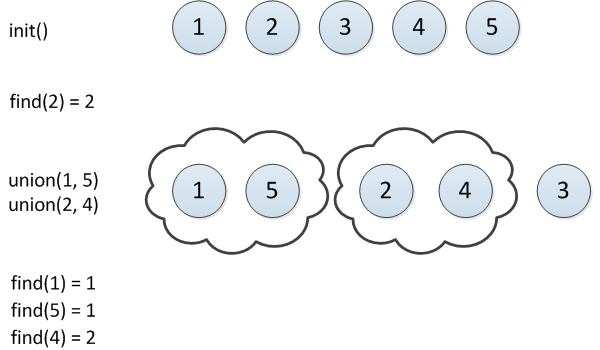
\includegraphics[width=0.6\linewidth]{img/DSU_1_Example.png}
    \label{union-find}
\end{center}

\subsection{Наивная реализация}
\begin{enumerate}
    \item Создаем массив с индексами от 1 до $N$
    \begin{itemize}
        \item Индекс означает номер элемента
        \item Значение по индексу — номер множества, к которому относится элемент
    \end{itemize}
    \item Операция \code{find(x)}
    \begin{itemize}
        \item Нужно вернуть содержимое ячейки с номером $x$
        \item \textbf{Сложность} — $O(1)$
    \end{itemize}
    \item Операция \code{union(x, y)}
    \begin{itemize}
        \item Узнаем номера множеств, содержащих эти элементы (пусть это $a$ и $b$ соответственно)
        \item Проходим по всему массиву и заменяем значения $b$ на $a$
        \item \textbf{Сложность одной операции} — $O(N)$
        \item \textbf{Сложность объединения всех множеств} — $O(N^2)$
    \end{itemize}
\end{enumerate}

\subsection{Реализация с использованием линейных списков}
Идея этой реализации заключается в том, что мы заводим второй массив, на индексах которого стоят номера множеств, а по индексу хранится список элементов соответствующего множества

Тогда при вызове \code{union(x, y)} мы делаем так: \code{max(x, y) += min(x, y)}

\subsubsection*{Сложность}
Так как мы храним второй массив, то мы \textit{тратим больше памяти}, однако алгоритм будет работать \textit{быстрее}, за $O(N\log N)$, так как делаем $O(\log N)$ шагов на каждом шаге $O(N)$ для объединения множеств

\begin{center}
    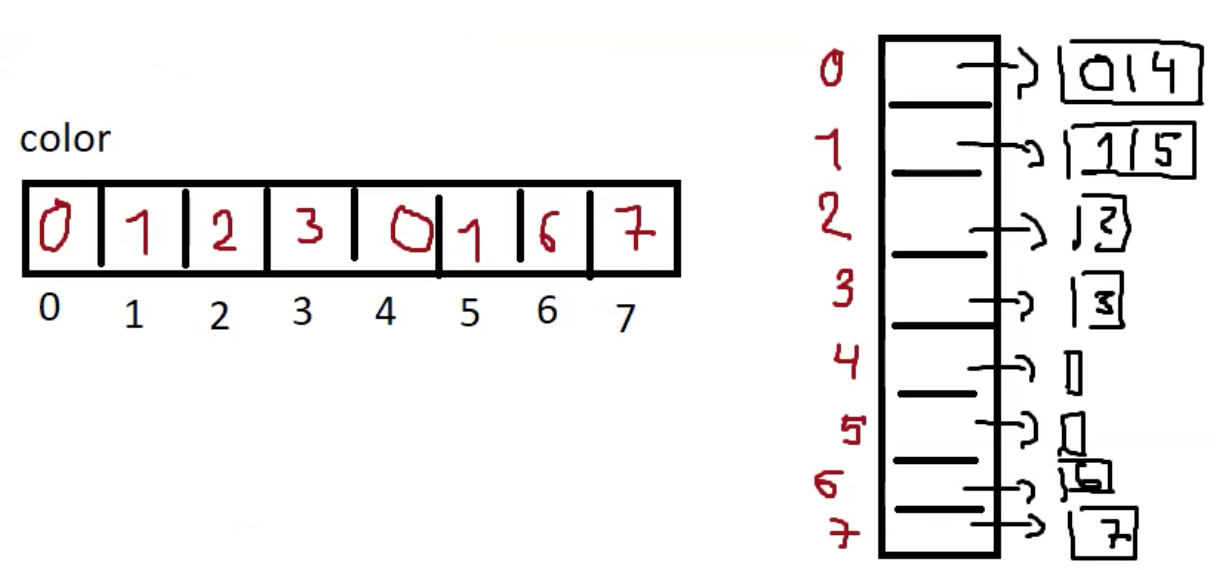
\includegraphics[width=0.75\linewidth]{img/linlist2.png}
    \label{union-find-lin}
\end{center}

\subsection{Система непересекающихся множеств}
Идея заключается в хранении каждого множества в виде дерева

Мы имеем единственный массив предков \code{p}. Индексы в нем — номера элементов, а по индексу хранится номер предка

\begin{center}
    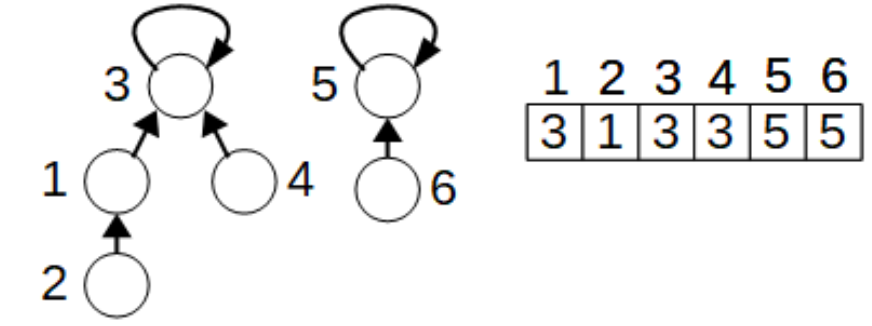
\includegraphics[width=0.6\linewidth]{img/snm.png}
    \label{dsu}
\end{center}

Петля у вершины означает, что вершина является корнем дерева, а в \code{p} на позицию с номером корня записывается значение самого корня

Вместо этого, в \code{p} на позицию корня можно поставить $-1$, суть не изменится

Тогда операции \code{find(x)} и \code{union(x, y)} можно реализовать так:

\begin{lstlisting}
    int find(x){
        while (p[v] != -1){
            v = p[v]
        }
        return v
    }
    
    void union(x, y){
        p[find(x)] = find(y)
    }
\end{lstlisting}

\textbf{Сложность} — $O(N^2)$

\subsubsection{Сжатие путей}
Идея заключается в том, что после поиска корня множества с помощью \code{find(x)} мы записываем этот корень в \code{parent} для вершины $x$ и всех вершин, пройденных по пути

Теперь в массиве предков для каждой вершины там может храниться не непосредственный предок, а предок предка, предок предка предка, и т.д

\textbf{Сложность} — $O(\log N)$

\subsubsection{Объединение деревьев}
Идея: нужно подвешивать дерево с большей глубиной к дереву с меньшей глубиной

Для каждого дерева храним его глубину в массиве

\textbf{Сложность} — $O(\log N)$

\subsection{Алгоритм Краскала}
\begin{itemize}
    \item Отсортируем все рёбра по возрастанию
    \item Каждая вершина находится в своем отдельном множестве
    \item В остовное дерево берем те рёбра, которые соединяют разные множества вершин
    \item При добавлении ребра происходит объединение множеств
\end{itemize}

Алгоритм используется для построения минимального остовного дерева в графе

Реализовать представленный алгоритм проще всего с помощью СНМ. Необходимо отсортировать рёбра по неубыванию по их весам. Далее мы каждую вершину можем поместить в свое собственное дерево, то есть, создаем некоторое множество подграфов. Дальше итерируемся по всем рёбрам в отсортированном порядке и смотрим, принадлежат ли инцидентные вершины текущего ребра разным подграфам с помощью функции find() или нет, если оба конца лежат в разных компонентах, то объединяем два разных подграфа в один с помощью функции union().

Итоговая сложность составит $O(E\log V+V+E)=O(E\log V)$, где $O(E\log V)$ - сортировка, $O(V)$ — создание отдельных множеств, $O(1)$ — find() и union()

\newpage
\section{Дерево отрезков}
\subsection{Дерево отрезков}
Дан массив $a$ из $n$ целых чисел, и требуется отвечать на запросы двух типов:

\begin{enumerate}
    \item Изменить значение в ячейке (т. е. реагировать на присвоение \code{a[k] = x})
    \item Вывести сумму элементов $a_i$ на отрезке с $l$ по $r$
\end{enumerate}

Построим вспомогательное дерево

\begin{itemize}
    \item Посчитаем сумму всего массива и сохраним ее
    \item Разделим его пополам, посчитаем сумму на половинах и тоже сохраним
    \item Каждую половину разделим пополам ещё раз, и т.д., пока не придём к отрезкам длины 1
\end{itemize}

\begin{center}
    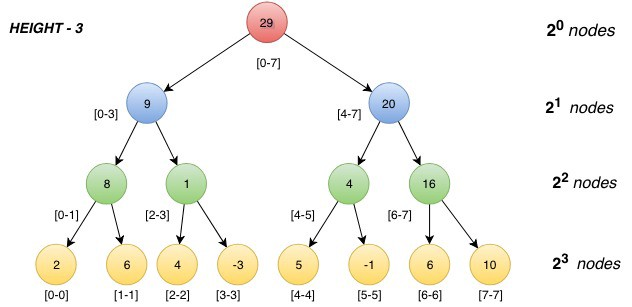
\includegraphics[width=0.9\linewidth]{img/segtree-example.jpg}
    \label{segtree-ex}
\end{center}

Корень этого дерева соответствует отрезку $[0, n)$, а каждая вершина (не считая листьев) имеет ровно двух сыновей, которые тоже соответствуют каким-то отрезкам

\subsection{Операции на отрезке}
Здесь представлены операции на отрезке, реализованные с помощью указателей. Эта реализация не самая эффективная, но самая простая, решающая большинство задач. Подробнее о других реализациях \href{http://e-maxx.ru/algo/segment_tree}{тут} и \href{https://codeforces.com/blog/entry/18051}{тут}
% Можно ввести нумерацию вершин и расположить их в массиве, подробнее об этом \href{http://e-maxx.ru/algo/segment_tree}{тут} и \href{https://codeforces.com/blog/entry/18051}{тут}

\subsubsection{Построение}
Строить дерево отрезков можно рекурсивным конструктором, который создает детей, пока не доходит до листьев

Если изначально массив не нулевой, то можно сразу при построении вычислять суммы

\textbf{Сложность} — $O(n)$

\begin{lstlisting}
Segtree(int lb, int rb) : lb(lb), rb(rb) {
    if (lb + 1 == rb)
        s = a[lb];
    else {
        int t = (lb + rb) / 2;
        l = new Segtree(lb, t);
        r = new Segtree(t, rb);
        s = l->s + r->s;
    }
}
\end{lstlisting}

\subsubsection{Изменение}
Для запроса прибавления будем рекурсивно спускаться вниз, пока не дойдем до листа, соответствующего элементу $k$, и на всех промежуточных вершинах прибавим $x$:

\begin{lstlisting}
void add(int k, int x) {
    s += x;
    if (l){
        if (k < l->rb)
            l->add(k, x);
        else
            r->add(k, x);
    }
}
\end{lstlisting}

\textbf{Сложность} — $O(\log n)$

\subsubsection{Сумма}
Нужно делать разбор случаев, как отрезок запроса пересекается с отрезком вершины:

\begin{enumerate}
    \item Если лежит полностью в отрезке запроса, вывести сумму
    \item Если не пересекается с отрезком запроса, вывести ноль
    \item Иначе: рекурсивно запускаемся от детей
\end{enumerate}

\begin{lstlisting}
int sum(int lq, int rq) {
    if (lb >= lq && rb <= rq)
        return s;
    if (max(lb, lq) >= min(rb, rq))
        return 0;
    return l->sum(lq, rq) + r->sum(lq, rq);
}
\end{lstlisting}

\textbf{Сложность} — $O(\log n)$. На каждом уровне дерева отрезков наша рекурсивная функция может посетить максимум четыре отрезка; тогда, учитывая оценку $O(\log n)$ для высоты дерева, мы получаем асимптотику времени работы алгоритма


\subsection{Применение дерева отрезков}
Дерево отрезков может применяться в таких задачах, как

\begin{itemize}
    \item поиск суммы на подотрезке
    \item поиск минимума/максимума на отрезке
    \item массовые изменения массивов (например, прибавление значения ко всем элементам отрезка)
\end{itemize}

\newpage
\section{Дерево поиска}
\textbf{\textit{Бинарное дерево поиска}} — дерево, для которого выполняются следующие свойства:

\begin{itemize}
    \item У каждой вершины не более двух детей
    \item Все вершины обладают \textit{ключами}, на которых определена операция сравнения (например, целые числа или строки)
    \item У всех вершин \textit{левого} поддерева вершины $v$ ключи \textit{не больше}, чем ключ $v$
    \item У всех вершин \textit{правого} поддерева вершины $v$ ключи \textit{больше}, чем ключ $v$
    \item Оба поддерева — левое и правое — являются бинарными деревьями поиска
\end{itemize}

В \textit{небинарных} деревьях количество детей может быть больше двух, и при этом в «более левых» поддеревьях ключи должны быть меньше, чем «более правых»

Для работы с деревьями поиска нужно создать структуру

\begin{lstlisting}
struct Node:
  T key                    // key of the node
  Node left                // pointer to the left child
  Node right               // pointer to the right child
  Node parent              // pointer to the parent
\end{lstlisting}

\subsection{Поиск элемента}
Нужна функция, принимающая корень дерева и искомый ключ

\begin{itemize}
    \item Для каждого узла сравниваем значение его ключа с искомым ключом
    \item Если ключи одинаковы, то функция возвращает текущий узел
    \item В противном случае функция вызывается рекурсивно для левого или правого поддерева
\end{itemize}

\begin{lstlisting}
Node search(x : Node, k : T):
   if x == null or k == x.key
      return x
   if k < x.key
      return search(x.left, k)
   else
      return search(x.right, k)
\end{lstlisting}

\textbf{Сложность в худшем случае} — $O(h)$ ($h$ — высота дерева), так как узлы, которые посещает функция образуют нисходящее дерево. Такое возможно, когда дерево является «бамбуком»

\textbf{Сложность в сбалансированном дереве} — $O(\log N)$, потому что высота такого дерева равна $O(\log N)$

\subsection{Вставка элемента}
Почти то же самое, что поиск элемента, но теперь, когда у текущей вершины нет нужного ребенка, нужно подвесить на нее вставляемый элемент

\begin{lstlisting}
Node insert(x : Node, z : T):               // x - root of the subtree, z - key to be inserted
   if x == null 
      return Node(z)                        // attach a Node with key = z
   else if z < x.key
      x.left = insert(x.left, z)
   else if z > x.key
      x.right = insert(x.right, z)
   return x
\end{lstlisting}

\subsection{Удаление элемента}
Рассмотрим три случая при рекурсивной реализации

\begin{enumerate}
    \item Удаляемый элемент находится в \textit{левом} поддереве текущего поддерева
    \begin{itemize}
        \item тогда нужно рекурсивно удалить элемент из нужного поддерева
    \end{itemize}
    \item Удаляемый элемент находится в \textit{правом} поддереве
    \begin{itemize}
        \item тогда нужно рекурсивно удалить элемент из нужного поддерева
    \end{itemize}
    \item Удаляемый элемент находится в \textit{корне}; есть два случая:
    \begin{itemize}
        \item у него два дочерних узла
        \begin{itemize}
            \item нужно заменить его минимальным элементом из правого поддерева и рекурсивно удалить этот минимальный элемент из правого поддерева
        \end{itemize}
        \item у него один дочерний узел
        \begin{itemize}
            \item нужно заменить удаляемый элемент потомком
        \end{itemize}
    \end{itemize}
\end{enumerate}

\begin{lstlisting}
Node delete(root : Node, z : T):    // root of subtree, key to delete
  if root == null
    return root
  if z < root.key
    root.left = delete(root.left, z)
  else if z > root.key
    root.right = delete(root.right, z)
  else if root.left != null and root.right != null
    root.key = minimum(root.right).key
    root.right = delete(root.right, root.key)
  else
    if root.left != null
      root = root.left
    else if root.right != null
      root = root.right
    else
      root = null
  return root
\end{lstlisting}
% \subsubsection*{Еще один вариант объяснения}
% \begin{enumerate}
%     \item Если пытаемся удалить лист или какую-то вершину в одном из поддеревьев, то все хорошо. Просто вырезаем вершину и на ее место ставим потомка и всех потомков потомка
%     \item Если же пытаемся удалить 
% \end{enumerate}

\newpage
\section{LCA (TBA)}

\end{document}
